\documentclass[border=10pt]{standalone}
\usepackage{tikz}\usepackage{amsmath}\usetikzlibrary{calc,arrows.meta}
\begin{document}
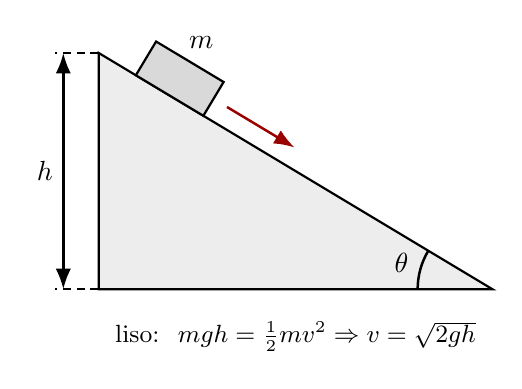
\begin{tikzpicture}[line width=0.9pt,>={Latex[length=2.6mm]}]
  \coordinate (A) at (0,0); \coordinate (B) at (5,0); \coordinate (C) at (0,3);
  \draw[thick,fill=black!7] (A)--(B)--(C)--cycle;
  % bloque SOBRE la pendiente, inclinado
  \begin{scope}[shift={($(C)!0.18!(B)$)},rotate=-30.96]
    \draw[thick,fill=black!15] (-0.5,0) rectangle (0.5,0.5);
    \node at (0,0.78){$m$};
    \draw[->,red!60!black] (0.7,0.25)--(1.7,0.25);   % desliza cuesta abajo
  \end{scope}
  % altura h
  \draw[densely dashed] (A)--($(A)+(-0.55,0)$); \draw[densely dashed] (C)--($(C)+(-0.55,0)$);
  \draw[<->] (-0.45,0)--(-0.45,3) node[midway,left]{$h$};
  % angulo theta en B
  \draw ($(B)+(180:0.95)$) arc (180:149:0.95); \node at ($(B)+(164:1.2)$){$\theta$};
  \node at (2.5,-0.6){\small liso: $\;mgh=\tfrac12 mv^2\Rightarrow v=\sqrt{2gh}$};
\end{tikzpicture}
\end{document}
